\chapter{Background}

\section{Argumentation Frameworks}


Argumentation frameworks were first formally described by Dung in 1995 \cite{DUNG1995321}. They represent an information state, where various conclusions can be drawen from. An AF $G = (A, R)$ consists of two parameters: a set of arguments $A$, and a collection of relations $R$, called attacks which describe the conflicts between the arguments.

They are mostly used in the fields of \ac{AI}, f.e. in automated reasoning and logic programming \cite{AFINAIARLP, AFINAIARLPexample}. But do also find their applications in other fields like Natural Language Processing \cite{AFINNLP}, Trust and Reputation Systems \cite{AFINTaRS}, and even in Game Theory and Strategic Reasoning \cite{AFinGames}.

AFs are represented by directed graph, where the nodes are an abstraction of the arguments $A$, and the arrows represent the attacks $R$. Let us define an AF $G = (A, R)$ with the arguments 
\texttt{A=\{a, b, c, d, e\}} and the attacks 
\texttt{R=[(a,b),}
\texttt{(b,b),}
\texttt{(a,c),}
\texttt{(c,a),}
\texttt{(c,d),}
\texttt{(d,e),}
\texttt{(e,d)]}. With the arguments and attacks, we can create a directed graph \ref{af:backgroundAFexample1}
\begin{figure}[h]
    \centering
    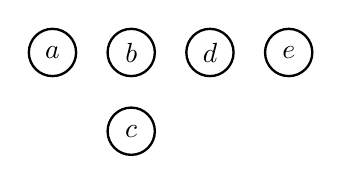
\begin{tikzpicture}
        % Singletons
        \def \ax{0}     \def \ay{0}
        \def \bx{1}     \def \by{0}
        \def \cx{1}     \def \cy{-1}
        \def \dx{2}     \def \dy{0}
        \def \ex{3}     \def \ey{0}

        \draw[line width=0.3mm] (\ax, \ay) circle (0.3) node[anchor=center]{$a$};
        \draw[line width=0.3mm] (\bx, \by) circle (0.3) node[anchor=center]{$b$};
        \draw[line width=0.3mm] (\cx, \cy) circle (0.3) node[anchor=center]{$c$};
        \draw[line width=0.3mm] (\dx, \dy) circle (0.3) node[anchor=center]{$d$};
        \draw[line width=0.3mm] (\ex, \ey) circle (0.3) node[anchor=center]{$e$};

        % Attacks
        \DrawAttackHorizontal{R}{\ax}{\ay}{\bx}{\by}
        \DrawSelfAttackRightSingleton{\bx}{\by}
        \DrawAttackDiagonal{NB}{\ax}{\ay}{\cx}{\cy}
        \DrawAttackDiagonal{PLR}{\cx}{\cy}{\dx}{\dy}
        \DrawAttackHorizontal{B}{\ex}{\ey}{\dx}{\dy}
    \end{tikzpicture}
    \caption{\ac{AF} G}
    \label{af:backgroundAFexample1}
\end{figure}

To be able to conclude something, out of an abstract AF, we need to define semantics. A semantic defines a subset of argument sets that satisfy the semantic-specific rules. Dung already defined different semantics \cite{Dung1995-DUNOTA-2} like \ac{cf}, \ac{adm} and \ac{stb}. According to Dungs definitions, a set \textit{S} is \ac{cf} if there are no attacks between the arguments in \textit{S}. The conflict-free set is mainly a building block for the other semantics, which means that the conflict-free set is always a superset of admissible and stable. In the example \ref{af:backgroundAFexample1} the $conflict-free$ sets are:
\texttt{\{a\}},
\texttt{\{c\}},
\texttt{\{d\}},
\texttt{\{e\}},
\texttt{\{a, d\}},
\texttt{\{a, e\}},
\texttt{\{c, e\}},


An admissible set is a conflict-free set, where each argument in \textit{S} has a defender in \textit{S}. In the example \ref{af:backgroundAFexample1} the $admissible$ sets are:
\texttt{\{a\}},
\texttt{\{c\}},
\texttt{\{e\}},
\texttt{\{a, d\}},
\texttt{\{a, e\}},
\texttt{\{c, e\}},

Finally, a stable set is a conflict-free set, if for every argument, which is not in \textit{S}, has an attacker which is in \textit{S}. In the example \ref{af:backgroundAFexample1} the $stable$ sets are:
\texttt{\{a, d\}},
\texttt{\{a, e\}},


The specific rules can be defined via a boolean formula. They can be used to encode the \acp{AF} to be solvable with different boolean solvers like \ac{ASP} \cite{DBLP:journals/corr/abs-1301-1388} or, as in our case, with a \ac{SAT-Solver} \cite{DBLP:journals/amai/AmgoudD13}. Unfortunately, drawing a conclusion from an AF can be challenging, e.g., it can be NP-complete and sometimes even be beyond NP to decide whether an argument is acceptable under a specific argumentation semantics \cite{DBLP:journals/ai/DvorakGRW23}.



\section{Clustering of Argumentation Frameworks}

When talking about AFs in general, we already have an abstraction layer due to the arguments abstraction. By clustering, we add another layer of abstraction where we combine different arguments into one or multiple so called \textit{clusters}. The arguments which are not clustered are called \textit{singletons}.
By definition, a cluster is a single entity (composed of multiple arguments) which can be integrated in an AF to reduce the complexity. While reducing the overall complexity of the AF with clusters, we add a new computation layer: Computing \textit{faithful} clustered AFs. The term \textit{faithful} describes the property of a clustered AF, that every abstract semantic extension can be mapped to a concrete semantic extension. If the clustered AF creates a semantic set which cannot be mapped to a concrete set, we call it \textit{spurious}. 

%\textit{TODO: Definition of Semantics}
Since clusters can not be treated the exact same way as an argument, we need to redefine the semantics. Let us consider a clustered AF $\hat{G}=(\hat{A}, \hat{R})$ and redefine the following semantics:
\paragraph{conflict-free:} A set of arguments is conflict-free, if there is no attack between the singletons of the set. Or, formally, as specified in \cite{DBLP:conf/kr/SaribaturW21}:

\begin{center}
$\hat{S} \in \hat{cf}(\hat{G})$ \textit{iff for each} $\hat{a}, \hat{b} \in$ \textit{singleton}($\hat{G}$) \textit{we have} $(\hat{a}, \hat{b}) \not\in \hat{R}$.
\end{center}

\paragraph{admissible:} A set of arguments is admissible, if it is conflict-free and if every singleton which is being attacked, has a defender. Or, formally, as specified in \cite{DBLP:conf/kr/SaribaturW21}:

\begin{center}
$\hat{S} \in \hat{adm}(\hat{G})$ \textit{iff} $\hat{S} \in \hat{cf}(\hat{G})$ \textit{and if} $\hat{a} \in \hat{E}$ \textit{with} $(\hat{b}, \hat{a}) \in \hat{R}$ \textit{with singleton}($\hat{a}$),

\textit{then there is a} $\hat{c} \in \hat{G}$ \textit{with} $(\hat{c}, \hat{b}) \in \hat{R}$
\end{center}

\paragraph{stable:} stable
\begin{center}
    $\hat{S} \in \hat{stb}(\hat{G})$ \textit{iff} $\hat{S} \in \hat{cf}(\hat{G}),  \hat{b} \not\in \hat{S}$ \textit{implies that there is an}
\end{center}





Let us have a look at a concrete example. The concrete AF $G = (A, R)$ has the following arguments \texttt{A=\{a, b, c, d, e\}} with these attacks:
\texttt{R=[(a,b),}
\texttt{(b,b),}
\texttt{(a,c),}
\texttt{(c,a),}
\texttt{(c,d),}
\texttt{(d,e),}
\texttt{(e,d)]}. 

With this definition we can define the graph \textit{G} in \ref{af:backgroundClusterExample1}.

Now we can group the arguments \texttt{\{a, b, c, d\}} together into one single cluster \textit{h'}. The arguments for the abstract AF $H = (B, S)$ would then be \texttt{B=\{h', e\}} with the according attacks:
\texttt{S=[(h', e),}
\texttt{(e, h'),}
\texttt{(h', h')]}. 

With this defintion we can build the abstract clustered graph \textit{H} in \ref{af:backgroundClusterExample2}


\vspace{0.3cm}
\begin{figure}[h]
\begin{minipage}{.5\textwidth}
    \centering
    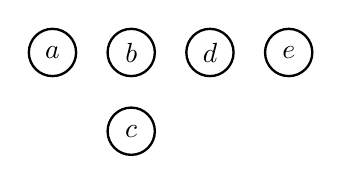
\begin{tikzpicture}
        % Singletons
        \def \ax{0}     \def \ay{0}
        \def \bx{1}     \def \by{0}
        \def \cx{1}     \def \cy{-1}
        \def \dx{2}     \def \dy{0}
        \def \ex{3}     \def \ey{0}

        \draw[line width=0.3mm] (\ax, \ay) circle (0.3) node[anchor=center]{$a$};
        \draw[line width=0.3mm] (\bx, \by) circle (0.3) node[anchor=center]{$b$};
        \draw[line width=0.3mm] (\cx, \cy) circle (0.3) node[anchor=center]{$c$};
        \draw[line width=0.3mm] (\dx, \dy) circle (0.3) node[anchor=center]{$d$};
        \draw[line width=0.3mm] (\ex, \ey) circle (0.3) node[anchor=center]{$e$};

        % Attacks
        \DrawAttackHorizontal{R}{\ax}{\ay}{\bx}{\by}
        \DrawSelfAttackRightSingleton{\bx}{\by}
        \DrawAttackDiagonal{NB}{\ax}{\ay}{\cx}{\cy}
        \DrawAttackDiagonal{PLR}{\cx}{\cy}{\dx}{\dy}
        \DrawAttackHorizontal{B}{\ex}{\ey}{\dx}{\dy}
    \end{tikzpicture}
    \caption{\ac{AF} G}
    \label{af:backgroundClusterExample1}
\end{minipage}%
\begin{minipage}{.5\textwidth}
    \centering
    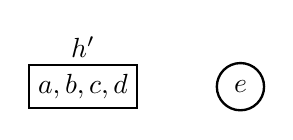
\begin{tikzpicture}
        % Singletons
        \def \ex{2}     \def \ey{0}
        \def \hx{0}     \def \hy{0}

        \node[rectangle, draw, line width=0.3mm] at (\hx, \hy) {$a,b,c,d$};
        \node at (0, 0.5) {$h'$};
        \draw[line width=0.3mm] (\ex, \ey) circle (0.3) node[anchor=center]{$e$};

        % Attacks
        \DrawSelfAttackLeftTopCluster{\hx-0.65}{\hy + 0.3}
        \DrawAttackHorizontal{B}{\ex}{\ey}{\hx+0.5}{\hy}
    \end{tikzpicture}
    \caption{\ac{AF} G' abstract}
    \label{af:backgroundClusterExample2}
\end{minipage}
\end{figure}

If we compare the stable sets of the concrete AF $G$ (e.g. \texttt{stb=[\{a, e\}, \{a, d\}]}) with the stable sets of the abstract clustered AF $H$ (e.g. \texttt{stb=[\{h'\}, \{e\}, \{e, h'\}]}), we see that it is spurious due to the stable set \texttt{\{e\}} which cannot be mapped to one of the concrete stable sets. To create a faithful clustered AF, we need to concretize one or more arguments of the cluster. By concretizing the argument \texttt{\{d\}}, we obtain a new AF $I=(B, T)$ with the arguments \texttt{B=\{h', d, e\}} and the attacks \texttt{T=[(h', d),}
\texttt{(d, e),}
\texttt{(e, d),}
\texttt{(h', h')]}. 

With this defintion we can build the concretized abstract graph \textit{I} in \ref{af:backgroundClusterExample3}


\begin{figure}[h]
    \centering
    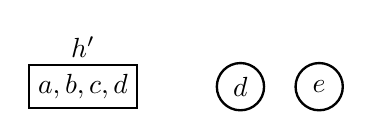
\begin{tikzpicture}
        % Singletons
        \def \ex{3}     \def \ey{0}
        \def \dx{2}     \def \dy{0}
        \def \hx{0}     \def \hy{0}

        \node[rectangle, draw, line width=0.3mm] at (\hx, \hy) {$a,b,c,d$};
        \node at (0, 0.5) {$h'$};
        \draw[line width=0.3mm] (\ex, \ey) circle (0.3) node[anchor=center]{$e$};
        \draw[line width=0.3mm] (\dx, \dy) circle (0.3) node[anchor=center]{$d$};

        % Attacks
        \DrawSelfAttackLeftTopCluster{\hx-0.65}{\hy + 0.3}
        \DrawAttackHorizontal{R}{\hx+0.5}{\hy}{\dx}{\dy}
        \DrawAttackHorizontal{B}{\ex}{\ey}{\dx}{\dy}
    \end{tikzpicture}
    \caption{\ac{AF} H' clustered}
    \label{af:backgroundClusterExample3}
\end{figure}

Every stable set in \ref{af:backgroundClusterExample3} (e.g. \texttt{\{d, h'\}, \{e, h'\}}) can be mapped to one of concrete stable sets of $G$, which means that the clustered AF $H'$ is faithful.




%\textit{TODO: Complexity}


\section{SAT-Solver}

\textit{TODO: What are SAT-Solvers}

\textit{TODO: Complexity of SAT-Problems}

\textit{TODO: Where and how do we use SAT-Solvers in the research}

